% =====================================================================
%  Άσκηση 5 (Bonus) — DS-CDMA/Rake & OFDM
%  Ασύρματες Επικοινωνίες, Πολυτεχνείο Κρήτης
%  Μεταγλώττιση:  xelatex report.tex   (δύο φορές)
% =====================================================================
\documentclass[11pt,a4paper]{article}

\usepackage{fontspec}
\usepackage{polyglossia}
\setmainlanguage{greek}
\setotherlanguage{english}
\setmainfont{Times New Roman}
\setsansfont{Arial}
\setmonofont{Consolas}
\newfontfamily\greekfont{Times New Roman}
\newfontfamily\greekfontsf{Arial}
\newfontfamily\greekfonttt{Consolas}
\newfontfamily\englishfont{Times New Roman}
\newfontfamily\englishfontsf{Arial}
\newfontfamily\englishfonttt{Consolas}

\usepackage{amsmath,amssymb}
\usepackage{graphicx}
\usepackage[margin=2.4cm]{geometry}
\usepackage{booktabs}
\usepackage{float}
\usepackage{caption}
\usepackage{enumitem}
\usepackage[hidelinks]{hyperref}

\captionsetup{font=small,labelfont=bf}
\setlength{\parindent}{0pt}
\setlength{\parskip}{4pt}
\graphicspath{{figures/}}
\emergencystretch=2em
\hyphenpenalty=1000
\setlength{\tabcolsep}{4.5pt}

% Μπλοκ παράθεσης του ζητουμένου της εκφώνησης
\newenvironment{zit}%
  {\begin{quote}\itshape}%
  {\end{quote}\noindent}

% Συντομεύσεις για την αγγλική τεχνική ορολογία
\newcommand{\en}[1]{\textenglish{#1}}
\newcommand{\dB}{\en{dB}}
\newcommand{\SNR}{\en{SNR}}
\newcommand{\BER}{\en{BER}}
\newcommand{\MRC}{\en{MRC}}
\newcommand{\Rake}{\en{Rake}}
\newcommand{\CP}{\en{CP}}

\begin{document}

% ---------------------------------------------------------------------
\begin{center}
  {\large\en{Technical University of Crete}}\\[2pt]
  {\large\en{School of Electrical and Computer Engineering}}\\[14pt]
  {\LARGE\bfseries Άσκηση 5 (\en{Bonus}) — \en{DS-CDMA/Rake} \& \en{OFDM}}\\[8pt]
  {\large Ασύρματες Επικοινωνίες}\\[14pt]
  \en{Student: Emmanouil Thomas Chatzakis}\\
  \en{StudentID: 2021030061}
\end{center}

\vspace{6pt}

Η υλοποίηση της άσκησης έγινε σε \en{Python} (\en{numpy}, \en{scipy}, \en{matplotlib}).
Ο κώδικας του πρώτου μέρους βρίσκεται στο \en{\texttt{cdma\_sim.py}}, του δεύτερου μέρους
στο \en{\texttt{ofdm\_sim.py}} και η κοινή υποδομή (θεωρητικές καμπύλες, εκτίμηση κλίσης,
σχήματα) στο \en{\texttt{common.py}}. Όλα τα αριθμητικά αποτελέσματα που παρατίθενται
παρακάτω είναι αναπαραγώγιμα με σπόρο τυχαιότητας ίσο με τον ΑΜ.

Η ορολογία και ο συμβολισμός ακολουθούν τις σημειώσεις του μαθήματος. Το πρώτο μέρος
αντιστοιχεί στο εδάφιο 4.2 του κεφαλαίου \emph{Διαφοροποίηση στις συχνότητες}
(\en{\texttt{Chapter\_Frequency\_\allowbreak Diversity\_1.pdf}}) και το δεύτερο στο κεφάλαιο
\en{\emph{OFDM}} (\en{\texttt{Chapter\_OFDM.pdf}}). Οι αριθμοί εξισώσεων που αναφέρονται
παρακάτω είναι αυτοί των αντίστοιχων κεφαλαίων.

Σε κάθε σημείο της καμπύλης \BER{} χρησιμοποιούμε \en{adaptive stopping}: η προσομοίωση
τρέχει μέχρι να συγκεντρωθούν τουλάχιστον $300$–$500$ σφάλματα ή μέχρι να εξαντληθεί το όριο
των δειγμάτων. Τα σημεία στα οποία καταγράφηκαν λιγότερα από $50$ σφάλματα τα θεωρούμε μη
μετρήσιμα και τα αποκλείουμε από την εκτίμηση της κλίσης, καθώς η σχετική τους αβεβαιότητα
($\sim 1/\sqrt{\text{σφάλματα}}$) θα αλλοίωνε το αποτέλεσμα. Τα σημεία αυτά σημειώνονται με
$^{\dagger}$ στους πίνακες.

% =====================================================================
\section{Πρώτο Μέρος — \en{DS-CDMA} και δέκτης \Rake{}}

\subsection*{Το μοντέλο}

Θεωρούμε το \en{uplink} ενός συστήματος \en{DS-CDMA} με $K$ σύγχρονους χρήστες. Κάθε
χρήστης εκπέμπει πακέτα $M=100$ δυαδικών ισοπίθανων συμβόλων $s_k[j] \in \{+1,-1\}$ και
χρησιμοποιεί \en{code} μήκους $N$,
\[
  c_k = \tfrac{1}{\sqrt{N}}\,\en{sign}\!\left(\en{randn}(N,1)\right),
  \qquad k = 1,\dots,K ,
\]
οπότε $\|c_k\|=1$. Το $N$ είναι το \en{processing gain} του συστήματος. Το \en{code} κάθε
χρήστη δημιουργείται \emph{μία φορά} και παραμένει σταθερό καθ' όλη τη διάρκεια του
πειράματος, όπως ζητά η εκφώνηση.

Η ροή \en{chips} του χρήστη $k$ είναι $x_k = s_k \otimes c_k$ (γινόμενο \en{Kronecker}),
δηλαδή κάθε σύμβολο απλώνεται σε $N$ \en{chips}. Το \en{wideband} κανάλι κάθε χρήστη έχει
μιγαδική κρουστική απόκριση μήκους $L$,
\[
  h_k \sim \mathcal{CN}\!\left(0, \tfrac{1}{L} I_L\right),
  \qquad \text{άρα}\qquad \mathbb{E}\!\left[\|h_k\|^2\right] = 1 ,
\]
σταθερή μέσα σε κάθε πακέτο και ανεξάρτητη από πακέτο σε πακέτο. Σύμφωνα με την εξ.~(4.10)
η έξοδος του καναλιού είναι
\[
  y_m \;=\; \sum_{k=1}^{K}\sum_{l=0}^{L-1} h_{k,l}\, x_k[m-l] \;+\; w_m ,
  \qquad w_m \sim \mathcal{CN}(0,\sigma_N^2),
\]
και ορίζουμε $\SNR_{\en{dB}} = 10\log_{10}\frac{1}{\sigma_N^2}$ (στις σημειώσεις η διασπορά
του θορύβου συμβολίζεται $N_0$).

Ακολουθώντας την εξ.~(4.12), για κάθε διάνυσμα $a$ ορίζουμε το ολισθημένο
$a^{(l)} := [\,0_l^T \ \ a^T \ \ 0_{L-1-l}^T\,]^T$. Τότε η εξ.~(4.13) δίνει
\[
  y \;=\; \sum_{l=0}^{L-1} h_l\, s\, c^{(l)} \;+\; w ,
\]
και το μπροστινό τμήμα του \Rake{} αποτελείται από $L$ \en{correlators}, έναν ανά
\en{finger}:
\[
  z_{j,l} \;=\; c_1^{(l)T}\, y \;=\; c_1^{T}\, y\!\left[jN+l \,:\, jN+l+N\right],
  \qquad l = 0,\dots,L-1 ,
\]
δηλαδή το \en{finger} $l$ «κοιτάζει» το παράθυρο του συμβόλου $j$ καθυστερημένο κατά $l$
\en{chips}.

Δύο σημεία όπου η προσομοίωσή μας είναι \emph{ακριβέστερη} από το μοντέλο των σημειώσεων:

\begin{enumerate}[leftmargin=2em]
  \item Η μετάδοση υλοποιείται με πλήρη γραμμική συνέλιξη της ροής \en{chips}, άρα
        \emph{δεν} κάνουμε την προσέγγιση της εξ.~(4.11), όπου οι $L-1$ πρώτες και
        τελευταίες εξισώσεις αγνοούν τη συνεισφορά του προηγούμενου και του επόμενου
        συμβόλου. Η \en{ISI} μεταξύ διαδοχικών συμβόλων μπαίνει αυτόματα στο μοντέλο.
  \item Η υπόθεση $c^{(l)T}c^{(m)} \approx 0$ της εξ.~(4.14) δεν επιβάλλεται, αλλά
        ελέγχεται αριθμητικά (εδάφιο~\ref{sec:orth} παρακάτω).
\end{enumerate}

Το ότι η καμπύλη \BER{} πέφτει παρ' όλα αυτά ακριβώς πάνω στη θεωρητική καμπύλη \MRC{}
δείχνει ότι οι προσεγγίσεις των σημειώσεων είναι απολύτως θεμιτές για $L \ll N$.

\subsection{Έλεγχος των υποθέσεων της εξ.~(4.14)}\label{sec:orth}

Η ανάλυση του \Rake{} στηρίζεται στις δύο υποθέσεις της εξ.~(4.14): $\|c\|=1$, που ισχύει
εξ ορισμού, και $c^{(l)T}c^{(m)} \approx 0$ για $l \neq m$, που ισχύει μόνο κατά προσέγγιση.
Μετράμε την \en{rms} τιμή της δεύτερης ποσότητας πάνω σε $4000$ τυχαία \en{codes}, και
παράλληλα τη διασυσχέτιση $c_1^{T}c_2$ δύο \emph{διαφορετικών} χρηστών, που είναι η πηγή της
\en{multi-user interference} του εδαφίου~1.4.

\begin{table}[H]
  \centering\small
  \begin{tabular}{cccc}
    \toprule
    $N$ & \en{rms} $|c^{(l)T}c^{(m)}|,\ l \neq m$ & \en{rms} $|c_1^{T}c_2|$ & $1/\sqrt{N}$ \\
    \midrule
    $32$  & $0.1696$ & $0.1765$ & $0.1768$ \\
    $64$  & $0.1227$ & $0.1239$ & $0.1250$ \\
    $128$ & $0.0877$ & $0.0874$ & $0.0884$ \\
    \bottomrule
  \end{tabular}
  \caption{\en{Numerical check of assumption (4.14): both correlations scale as
  $1/\sqrt{N}$.}}\label{tab:orth}
\end{table}

Παρατηρούμε ότι και οι δύο ποσότητες ακολουθούν σχεδόν ακριβώς το $1/\sqrt{N}$. Δηλαδή τα
\en{codes} δεν είναι ορθογώνια αλλά «σχεδόν ορθογώνια», και η ποιότητα της προσέγγισης
βελτιώνεται όσο μεγαλώνει το \en{processing gain} $N$. Αυτή η μοναδική παρατήρηση εξηγεί
ταυτόχρονα γιατί δουλεύει ο \Rake{} για $L \ll N$ \emph{και} γιατί η επίδοση υποβαθμίζεται
όταν προστίθενται χρήστες (εδάφιο~1.4).

\subsection{Δέκτης \Rake{} με $L$ \en{fingers} ($K=1$)}

\begin{zit}
Να υλοποιήσετε τον δέκτη \en{Rake} και να σχεδιάσετε το \BER{} για
$\SNR_{\en{dB}} = [0:2:20]$. Να σχεδιάσετε τις συναρτήσεις $f_i = 1/\SNR^i$, για
$i=1,2,3$, και να προσπαθήσετε να ανιχνεύσετε την τάξη \en{diversity} του σχήματος αυτού.
\end{zit}

Ο δέκτης του Σχήματος~4.3 των σημειώσεων συνδυάζει τις εξόδους των $L$ \en{correlators}
με \en{maximum ratio combining}. Κάθε \en{finger} δίνει, κατά την εξ.~(4.15),
\[
  \frac{|h_l|^2}{\|h\|}\,s + w'_l ,
  \qquad w'_l \sim \mathcal{CN}\!\left(0, \tfrac{|h_l|^2}{\|h\|^2} N_0\right),
\]
και το άθροισμά τους δίνει την εξ.~(4.16)
\[
  r_j \;=\; \frac{h_1^{H} z_j}{\|h_1\|} \;=\; \|h_1\|\,s_j + w'' ,
  \qquad w'' \sim \mathcal{CN}(0, N_0),
  \qquad
  \hat{s}_1[j] = \en{sign}\!\left(\en{Re}\{r_j\}\right).
\]
Αφού τα $h_l$ είναι \en{i.i.d.}, οι σημειώσεις προβλέπουν τάξη \en{diversity} ίση με $L$.

Για τη θεωρητική καμπύλη, το μέσο \SNR{} ανά \en{branch} είναι
\[
  \bar{\gamma} \;=\; \frac{\mathbb{E}\!\left[|h_{1,l}|^2\right]}{\sigma_N^2}
              \;=\; \frac{1/L}{\sigma_N^2}
              \;=\; \frac{\SNR}{L},
\]
δηλαδή το $1/L$ της διασποράς του καναλιού μετράει και δεν πρέπει να παραλειφθεί. Με $L$
\en{i.i.d.} \en{Rayleigh branches} ισχύει
\[
  P_e = \left(\frac{1-\mu}{2}\right)^{\!L}
        \sum_{k=0}^{L-1}\binom{L-1+k}{k}\left(\frac{1+\mu}{2}\right)^{\!k},
  \qquad \mu = \sqrt{\frac{\bar\gamma}{1+\bar\gamma}},
\]
με ασυμπτωτική μορφή $P_e \approx \binom{2L-1}{L} \big/ (4\bar\gamma)^L$.

\begin{figure}[H]
  \centering
  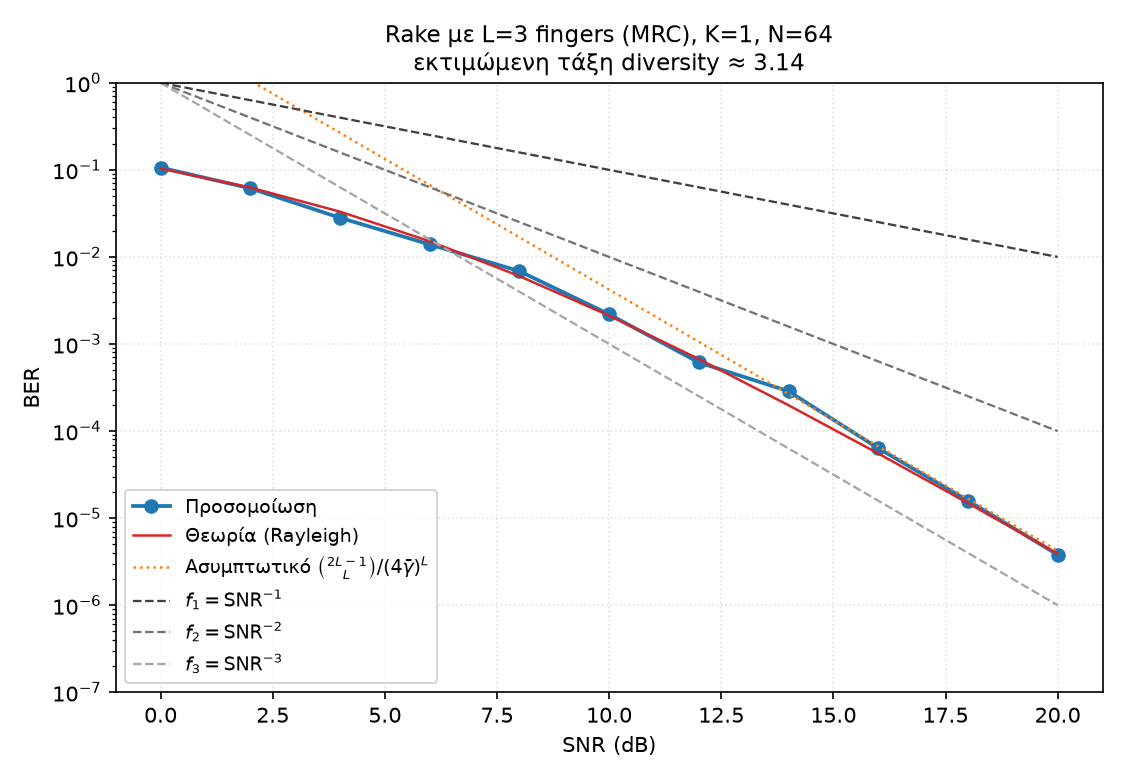
\includegraphics[width=0.49\textwidth]{A_mrc_L3_N64.png}%
  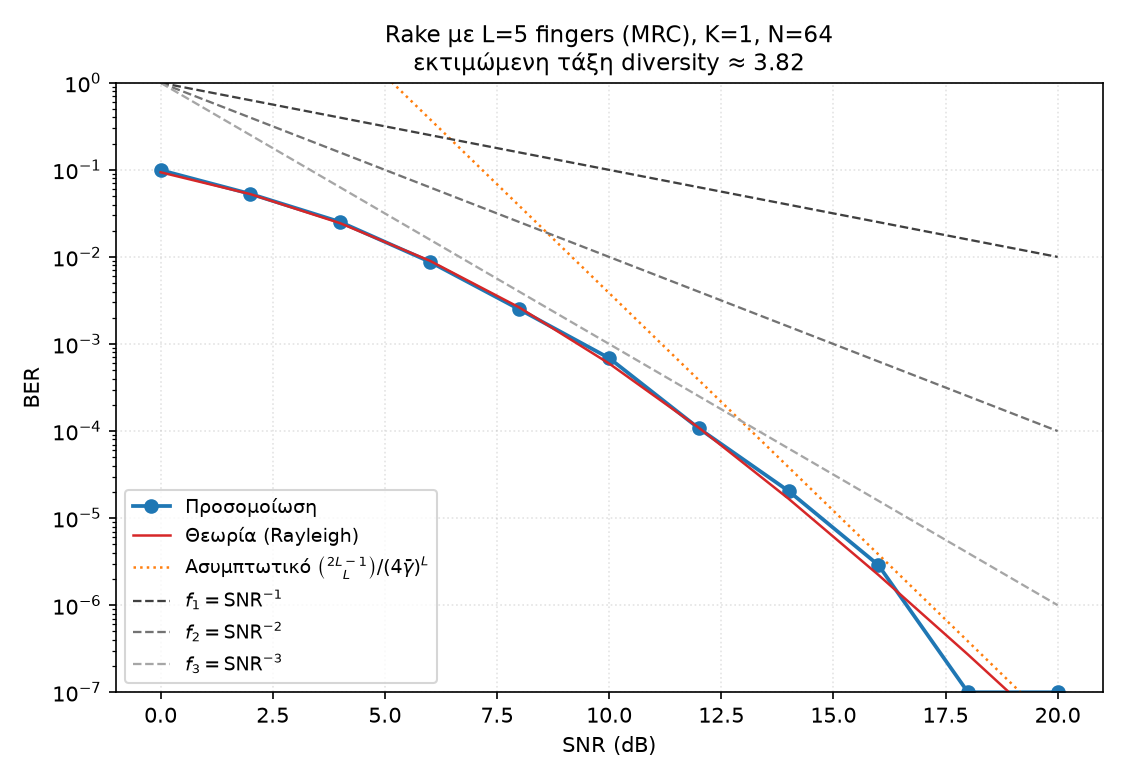
\includegraphics[width=0.49\textwidth]{A_mrc_L5_N64.png}
  \caption{\en{BER of the full Rake receiver ($L$ fingers, MRC), $K=1$, $N=64$.
  Left: $L=3$. Right: $L=5$.}}
\end{figure}

\begin{table}[H]
  \centering\small
  \begin{tabular}{lcccccc c}
    \toprule
    \SNR{} (\dB) & $0$ & $4$ & $8$ & $12$ & $16$ & $20$ & τάξη \en{diversity} \\
    \midrule
    $L=3$ & \texttt{1.06e-01} & \texttt{2.82e-02} & \texttt{6.86e-03} & \texttt{6.14e-04} & \texttt{6.35e-05} & \texttt{3.80e-06}$^{\dagger}$ & $\mathbf{3.14}$ \\
    $L=5$ & \texttt{9.93e-02} & \texttt{2.52e-02} & \texttt{2.50e-03} & \texttt{1.07e-04} & \texttt{2.90e-06}$^{\dagger}$ & — & $\mathbf{3.82}$ \\
    \bottomrule
  \end{tabular}
  \caption{\en{Full Rake (MRC): BER versus SNR and estimated diversity order.}}
\end{table}

Παρατηρούμε ότι η προσομοίωση πέφτει ακριβώς πάνω στη θεωρητική καμπύλη, γεγονός που
επικυρώνει ταυτόχρονα το μοντέλο του καναλιού, τους \en{correlators} και τον \en{combiner}
της εξ.~(4.16).

Για $L=3$ η κλίση της καμπύλης στα υψηλά \SNR{} είναι $3.14 \approx 3 = L$: η καμπύλη
\BER{} τρέχει παράλληλα στην $f_3 = \SNR^{-3}$ και τέμνει διαδοχικά τις $f_1$ και $f_2$.
Επιβεβαιώνεται δηλαδή η πρόβλεψη των σημειώσεων ότι ο \Rake{} με $L$ \en{fingers} εξάγει
τάξη \en{diversity} $L$.

Για $L=5$ η μετρούμενη κλίση είναι $3.82$ και όχι $5$. Αυτό δεν αποτελεί απόκλιση από τη
θεωρία: η τάξη \en{diversity} είναι \emph{ασυμπτωτική} έννοια και στο εύρος $0$–$20$~\dB{} η
κλίση δεν έχει προλάβει να συγκλίνει. Επιπλέον, για $L=5$ το \BER{} πέφτει κάτω από
$\sim 10^{-7}$ πριν από τα $20$~\dB{}, δηλαδή κάτω από το όριο μέτρησης των $10^{7}$
συμβόλων που επιτρέπει ο χρόνος εκτέλεσης.

\subsection{Δέκτης \Rake{} με $1$ \en{finger} ($K=1$)}

\begin{zit}
Να υλοποιήσετε δέκτη \en{Rake} με $1$ \en{finger} χρησιμοποιώντας μόνο τον πιο ισχυρό
συντελεστή του καναλιού κάθε φορά και να σχεδιάσετε το \BER{}. Να σχεδιάσετε τις συναρτήσεις
$f_i = 1/\SNR^i$, για $i=1,2,3$, και να προσπαθήσετε να ανιχνεύσετε την τάξη \en{diversity}
του σχήματος αυτού.
\end{zit}

Ο δέκτης αυτός (\en{selection combining}) κρατά μόνο τον ισχυρότερο συντελεστή, δηλαδή
ενεργοποιεί ένα μόνο από τα $L$ \en{fingers} του Σχήματος~4.3:
\[
  l^{\star} = \arg\max_{l} |h_{1,l}|,
  \qquad
  r_j = \frac{h_{1,l^\star}^{*}\, z_{j,l^\star}}{|h_{1,l^\star}|},
  \qquad
  \hat{s}_1[j] = \en{sign}\!\left(\en{Re}\{r_j\}\right).
\]
Η αντίστοιχη θεωρητική καμπύλη προκύπτει από την
$F_{\gamma_{\max}}(\gamma) = \left(1-e^{-\gamma/\bar\gamma}\right)^{L}$ και δίνει
\[
  P_e = \sum_{k=0}^{L-1} \binom{L-1}{k}(-1)^k \frac{L}{k+1}\cdot
        \frac{1}{2}\left(1-\sqrt{\frac{\bar\gamma_k}{1+\bar\gamma_k}}\right),
  \qquad \bar\gamma_k = \frac{\bar\gamma}{k+1}.
\]

\begin{figure}[H]
  \centering
  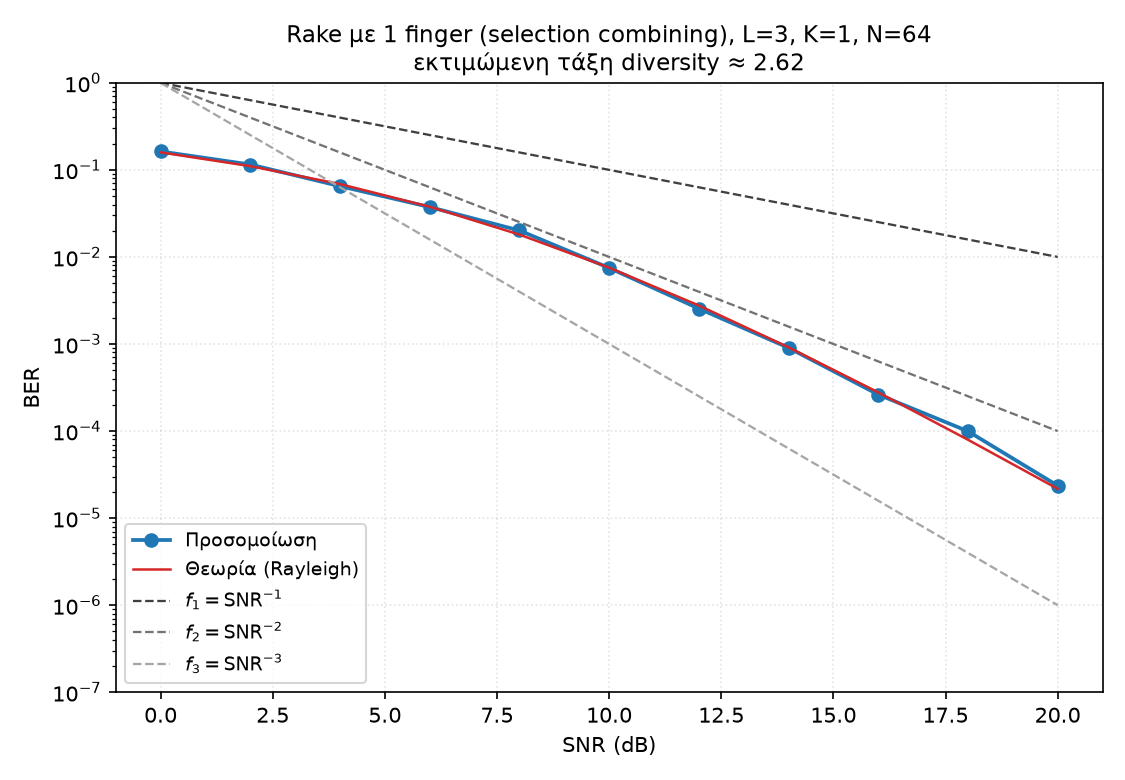
\includegraphics[width=0.49\textwidth]{A_sc_L3_N64.png}%
  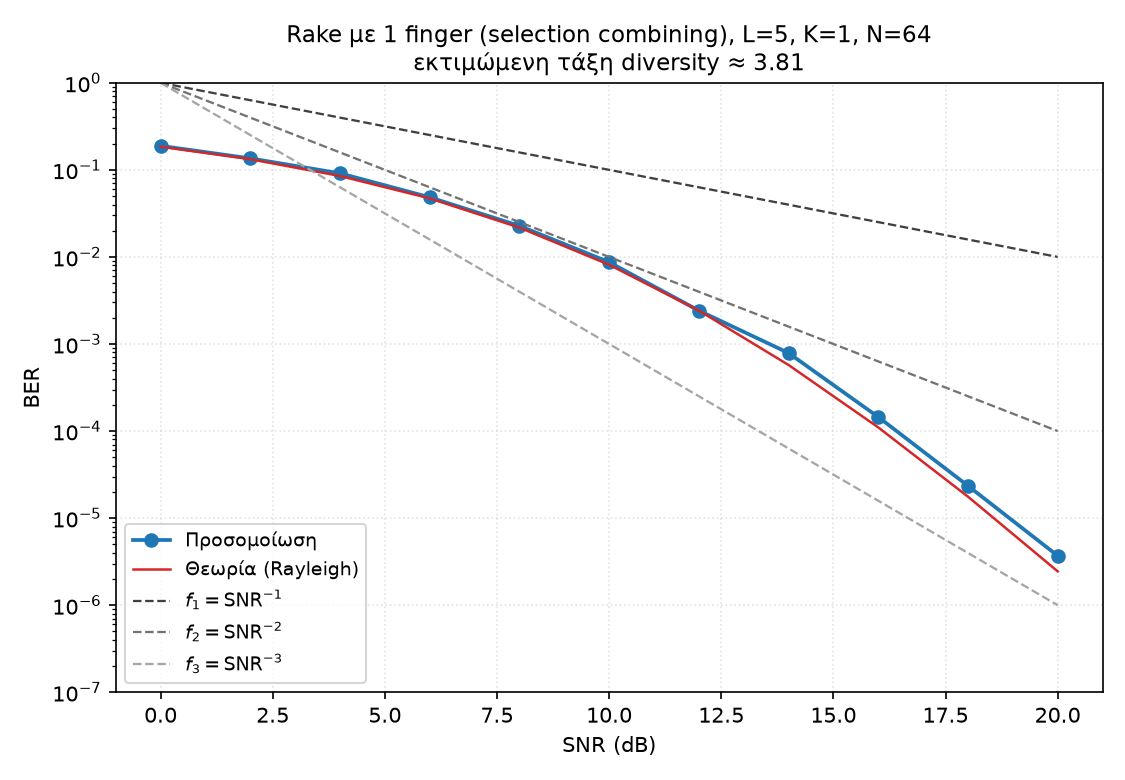
\includegraphics[width=0.49\textwidth]{A_sc_L5_N64.png}
  \caption{\en{BER of the 1-finger Rake (selection combining), $K=1$, $N=64$.
  Left: $L=3$. Right: $L=5$.}}
\end{figure}

\begin{figure}[H]
  \centering
  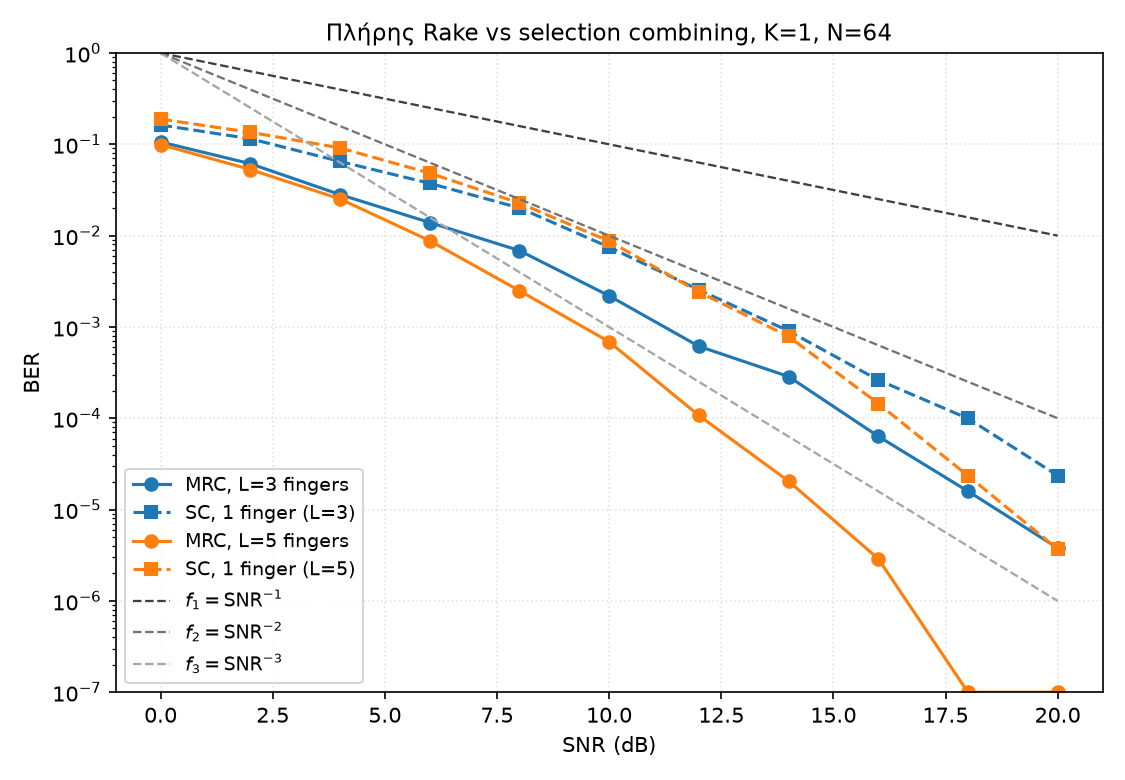
\includegraphics[width=0.72\textwidth]{A_mrc_vs_sc_N64.png}
  \caption{\en{Full Rake versus selection combining, $K=1$, $N=64$.}}
\end{figure}

\begin{table}[H]
  \centering\small
  \begin{tabular}{lcccccc c}
    \toprule
    \SNR{} (\dB) & $0$ & $4$ & $8$ & $12$ & $16$ & $20$ & τάξη \en{diversity} \\
    \midrule
    $L=3$ & \texttt{1.63e-01} & \texttt{6.50e-02} & \texttt{2.01e-02} & \texttt{2.55e-03} & \texttt{2.63e-04} & \texttt{2.36e-05} & $\mathbf{2.62}$ \\
    $L=5$ & \texttt{1.89e-01} & \texttt{9.13e-02} & \texttt{2.27e-02} & \texttt{2.42e-03} & \texttt{1.45e-04} & \texttt{3.70e-06}$^{\dagger}$ & $\mathbf{3.81}$ \\
    \bottomrule
  \end{tabular}
  \caption{\en{Selection combining: BER versus SNR and estimated diversity order.}}
\end{table}

Παρατηρούμε ότι το \en{selection combining} \emph{διατηρεί} την τάξη \en{diversity} $L$: η
κλίση παραμένει μεγάλη και σχεδόν ίδια με αυτήν του πλήρους \Rake{}. Ο λόγος είναι ότι
σφάλμα συμβαίνει μόνο όταν \emph{όλοι} οι $L$ συντελεστές βρεθούν ταυτόχρονα σε
\en{deep fade}, γεγονός με πιθανότητα $\sim \SNR^{-L}$ όπως και στο \MRC{}.

Αυτό που χάνεται δεν είναι το \en{diversity} αλλά το \en{array gain}. Στα $20$~\dB{} με
$L=3$ το \BER{} είναι $2.36\cdot10^{-5}$ έναντι $3.80\cdot10^{-6}$ του πλήρους \Rake{},
δηλαδή περίπου $6$ φορές χειρότερο ($\approx 3$~\dB{} απώλεια). Ο δέκτης με ένα \en{finger}
απλώς αγνοεί την ενέργεια των υπόλοιπων $L-1$ διαδρομών αντί να τη συνδυάσει, όπως κάνει η
εξ.~(4.16). Η μικρότερη μετρούμενη κλίση για $L=3$ ($2.62$ έναντι $3.14$) οφείλεται στο ότι
το \en{selection combining} συγκλίνει πιο αργά στην ασυμπτωτική του κλίση.

\subsection{Εισαγωγή δεύτερου χρήστη ($K=2$)}

\begin{zit}
Να χρησιμοποιήσετε τον \en{Rake} με $L$ \en{fingers} για την ανάκτηση της πληροφορίας του
πρώτου χρήστη. Να υπολογίσετε το \BER{} για $\SNR_{\en{dB}} = [0:2:16]$. Να συγκρίνετε το
\BER{} με αυτό του συστήματος με έναν χρήστη. Τι παρατηρείτε για διαφορετικά $N$;
\end{zit}

Στην ιδανική περίπτωση \en{AWGN} και ορθογώνιων \en{codes}, η εξ.~(4.9) των σημειώσεων δίνει
$r_k = c_k^{T} y = \|c_k\|^2 s_k + w'_k$, δηλαδή οι χρήστες διαχωρίζονται τέλεια. Εδώ όμως
τα \en{codes} είναι τυχαία και μόνο «σχεδόν ορθογώνια», με
$|c_1^{T}c_2| \sim 1/\sqrt{N}$ όπως μετρήσαμε στον Πίνακα~\ref{tab:orth}. Επαναλαμβάνουμε επομένως το
πείραμα με $L=3$ και $N = 32, 64, 128$, αποκωδικοποιώντας πάντα τον χρήστη~1 με τον πλήρη
\Rake{}.

\begin{figure}[H]
  \centering
  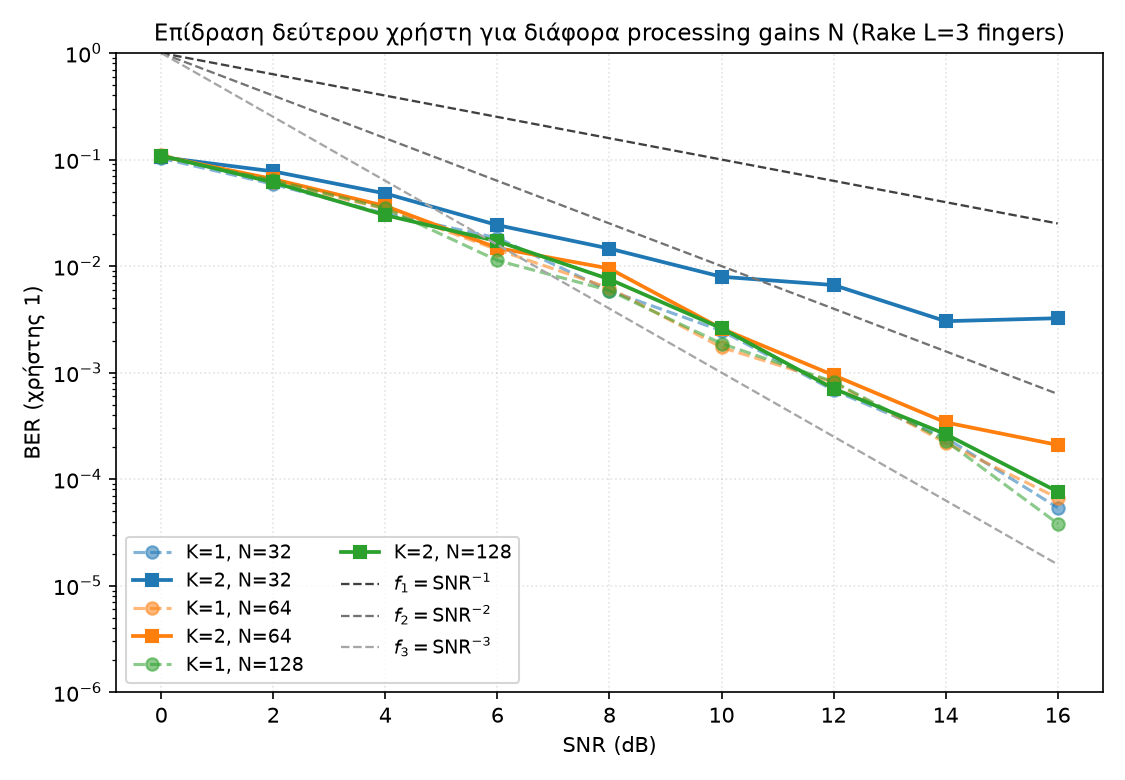
\includegraphics[width=0.78\textwidth]{A_K2_vs_K1_L3.png}
  \caption{\en{Effect of a second user for different processing gains $N$
  ($L=3$ fingers).}}
\end{figure}

\begin{table}[H]
  \centering\small
  \begin{tabular}{lcccc}
    \toprule
    $N$ & \BER{} ($K=1$) & \BER{} ($K=2$) & τάξη \en{div.} ($K=1$) & τάξη \en{div.} ($K=2$) \\
    \midrule
    $32$  & \texttt{5.40e-05} & \texttt{3.24e-03} & $2.75$ & $\mathbf{0.78}$ \\
    $64$  & \texttt{6.67e-05} & \texttt{2.10e-04} & $2.71$ & $\mathbf{1.63}$ \\
    $128$ & \texttt{3.83e-05} & \texttt{7.63e-05} & $3.33$ & $\mathbf{2.42}$ \\
    \bottomrule
  \end{tabular}
  \caption{\en{BER of user 1 at $16$~dB and estimated diversity order.}}
\end{table}

Ο δεύτερος χρήστης εισάγει \en{multi-user interference (MUI)}, ακριβώς επειδή δεν ισχύει η
ιδανική συνθήκη $c_i \perp c_j$ της εξ.~(4.9): η διασυσχέτιση είναι τάξης $1/\sqrt{N}$ και
όχι μηδέν. Η \en{MUI} είναι ανάλογη της ισχύος του σήματος και όχι του θορύβου, άρα
\emph{δεν} μειώνεται όταν αυξάνεται το \SNR{}.

Συνέπεια αυτού είναι η εμφάνιση \en{error floor}. Για $N=32$ το \BER{} «κολλάει» γύρω στο
$3\cdot10^{-3}$ μετά τα $12$~\dB{} και η φαινόμενη τάξη \en{diversity} καταρρέει από $2.75$
σε $0.78$: το \en{diversity} ουσιαστικά χάνεται.

Όσο μεγαλώνει το $N$, τόσο μικραίνει η \en{MUI} — η ισχύς της πέφτει $\sim 1/N$, δηλαδή
περίπου $3$~\dB{} ανά διπλασιασμό του $N$, σε πλήρη συμφωνία με τον Πίνακα~\ref{tab:orth}. Για $N=128$ η
καμπύλη του $K=2$ πρακτικά ταυτίζεται με αυτήν του $K=1$ ($7.63\cdot10^{-5}$ έναντι
$3.83\cdot10^{-5}$) και η τάξη \en{diversity} επανέρχεται στο $2.42$. Το \en{processing gain}
$N$ είναι επομένως αυτό που «αγοράζει» ανοχή σε πολλαπλούς χρήστες, με τίμημα το
\en{bandwidth} — ακριβώς το \en{trade-off} που περιγράφει το εδάφιο~4.2 των σημειώσεων.

\subsection{Περισσότεροι χρήστες ($K = 1,\dots,5$)}

\begin{zit}
Στη συνέχεια, να εισάγετε περισσότερους χρήστες. Τι παρατηρείτε;
\end{zit}

\begin{figure}[H]
  \centering
  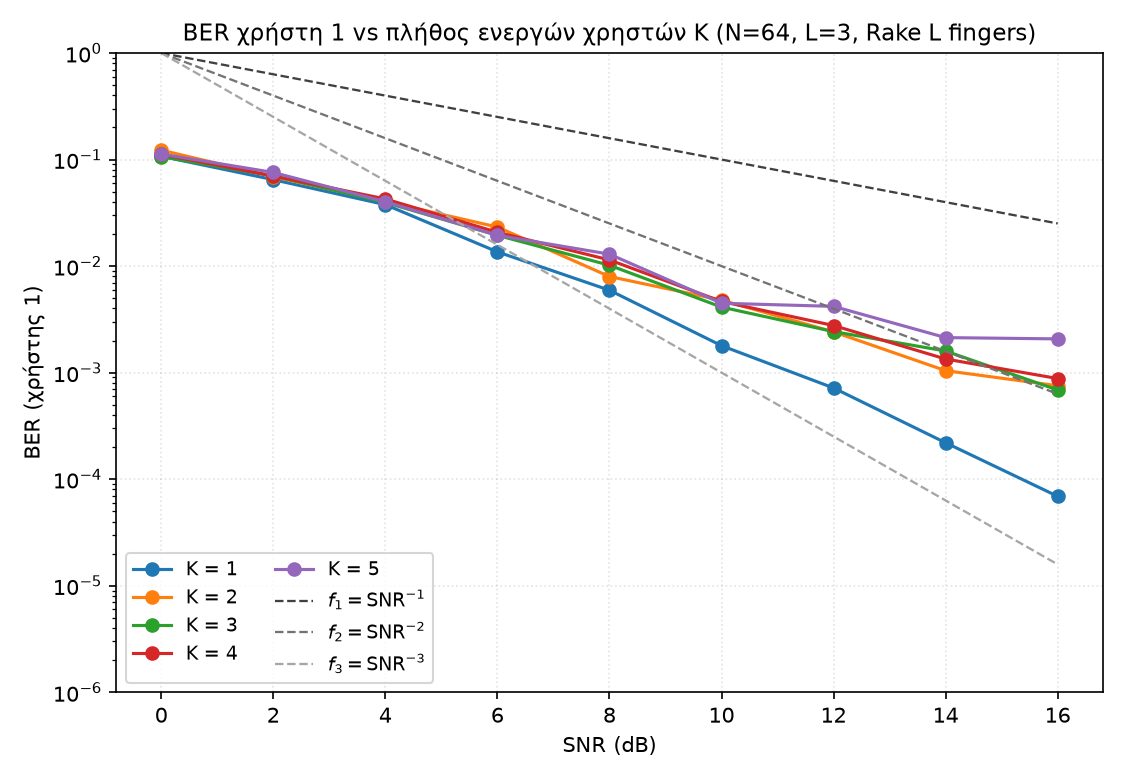
\includegraphics[width=0.78\textwidth]{A_manyusers_N64_L3.png}
  \caption{\en{BER of user 1 versus the number of active users $K$ ($N=64$, $L=3$).}}
\end{figure}

\begin{table}[H]
  \centering\small
  \begin{tabular}{lccccc}
    \toprule
    $K$ & $1$ & $2$ & $3$ & $4$ & $5$ \\
    \midrule
    \BER{} στα $16$~\dB{} & \texttt{6.90e-05} & \texttt{7.53e-04} & \texttt{6.87e-04} & \texttt{8.80e-04} & \texttt{2.07e-03} \\
    τάξη \en{diversity} & $2.54$ & $1.26$ & $1.37$ & $1.24$ & $0.76$ \\
    \bottomrule
  \end{tabular}
  \caption{\en{BER of user 1 at $16$~dB and estimated diversity order versus $K$
  ($N=64$, $L=3$).}}
\end{table}

Παρατηρούμε ότι η υποβάθμιση είναι δραματική στο πέρασμα από $K=1$ σε $K=2$ (μία τάξη
μεγέθους στο \BER{}) και πολύ πιο ήπια στη συνέχεια. Αυτό είναι αναμενόμενο: η συνολική
\en{MUI} αυξάνεται περίπου γραμμικά με το $K-1$, οπότε κάθε επιπλέον χρήστης προσθέτει όλο
και μικρότερο \emph{σχετικό} ποσοστό παρεμβολής.

Η τάξη \en{diversity} πέφτει σταθερά προς το $1$ και κάτω, δηλαδή για $K \ge 2$ το σύστημα
γίνεται \en{interference-limited} και όχι \en{noise-limited}. Σε αυτό το καθεστώς η αύξηση
της ισχύος εκπομπής δεν βοηθά, αφού και οι δύο όροι (σήμα και παρεμβολή) αυξάνονται μαζί.

Ο απλός δέκτης \Rake{} μεταχειρίζεται τους άλλους χρήστες ως θόρυβο, όπως ακριβώς
προαναγγέλλουν οι σημειώσεις στο τέλος του εδαφίου~4.2.1. Για να υποστηριχθούν περισσότεροι
χρήστες χρειάζεται είτε μεγαλύτερο \en{processing gain} $N$, είτε \en{multi-user detection}
(\en{decorrelator}, \en{MMSE}, \en{successive interference cancellation}).

% =====================================================================
\section{Δεύτερο Μέρος — διαμόρφωση \en{OFDM}}

\subsection*{Απόδειξη του ορισμού του \SNR{}}

\begin{zit}
Να αποδείξετε ότι το μέσο λαμβανόμενο \SNR{} σε \dB{} είναι
$\SNR_{\en{dB}} := 10\log_{10}\frac{2}{\sigma_n^2}$, όπου $\sigma_n^2$ είναι η ισχύς του
προσθετικού θορύβου.
\end{zit}

Μετά την αφαίρεση του \en{cyclic prefix} και τον \en{DFT}, κάθε \en{subcarrier} δίνει, κατά
την εξ.~(4.14),
\[
  \tilde{y}'_n = \tilde{h}_n\,\tilde{d}_n + \tilde{w}_n,
  \qquad \tilde{w}_n \sim \mathcal{CN}(0,\sigma_n^2).
\]
\begin{enumerate}[label=(\alph*),leftmargin=2em]
  \item \textbf{Ισχύς συμβόλου.} $\tilde d = \pm 1 \pm j \Rightarrow
        \mathbb{E}\!\left[|\tilde d|^2\right] = 1 + 1 = 2$.
  \item \textbf{Ισχύς καναλιού.} Από την εξ.~(4.15),
        $\tilde h_n = \sum_{l=0}^{L-1} h_l e^{-j2\pi ln/N_c}$ με $h_l$ ανεξάρτητα και
        μηδενικής μέσης τιμής, οπότε οι σταυρωτοί όροι μηδενίζονται:
        \[
          \mathbb{E}\!\left[|\tilde h_n|^2\right]
          = \sum_{l=0}^{L-1}\mathbb{E}\!\left[|h_l|^2\right] = L\cdot\frac{1}{L} = 1 .
        \]
  \item \textbf{Ισχύς θορύβου.} $\mathbb{E}\!\left[|\tilde w_n|^2\right] = \sigma_n^2$.
\end{enumerate}
Επομένως το μέσο λαμβανόμενο \SNR{} ανά \en{subcarrier} είναι
\[
  \SNR = \frac{\mathbb{E}\!\left[|\tilde h_n|^2\right]\,
               \mathbb{E}\!\left[|\tilde d_n|^2\right]}
              {\mathbb{E}\!\left[|\tilde w_n|^2\right]}
       = \frac{2}{\sigma_n^2},
  \qquad\text{δηλαδή}\qquad
  \SNR_{\en{dB}} = 10\log_{10}\frac{2}{\sigma_n^2}. \qquad \blacksquare
\]

Το βήμα (γ) απαιτεί προσοχή. Η υποσημείωση~1 της εξ.~(4.11) των σημειώσεων επισημαίνει ότι
η υλοποίηση του \en{DFT} σε \en{MATLAB} (και σε \en{numpy}) δεν πολλαπλασιάζει με
$1/\sqrt{N_c}$ στον ευθύ μετασχηματισμό, ενώ πολλαπλασιάζει με $1/N_c$ στον αντίστροφο, τη
στιγμή που ο ορισμός των σημειώσεων απαιτεί $1/\sqrt{N_c}$ \emph{και στις δύο} κατευθύνσεις.
Γι' αυτό καλούμε παντού τον \emph{ορθοκανονικό} \en{DFT}. Με τη σύμβαση αυτή ο λευκός
θόρυβος του πεδίου χρόνου παραμένει λευκός με την \emph{ίδια} διασπορά στο πεδίο συχνότητας,
το βήμα (γ) ισχύει ακριβώς και ο παραπάνω ορισμός δεν χρειάζεται διόρθωση κατά έναν
παράγοντα $N_c$. Αντίθετα, το $\tilde h_n$ της εξ.~(4.15) είναι η δειγματοληπτημένη απόκριση
συχνότητας του καναλιού και υπολογίζεται με \emph{μη} κανονικοποιημένο \en{DFT} — ο
συνδυασμός των δύο είναι που κάνει την εξ.~(4.14) να ισχύει ακριβώς.

\subsection{Κανάλι, είσοδος \en{4-QAM} και μετάδοση \en{OFDM}}

\begin{zit}
Να δημιουργήσετε τυχαίο μιγαδικό κανάλι $h_l$, $l=0,\dots,L-1$, με $h_l$ ανεξάρτητα όμοια
κατανεμημένα, $h_l \sim \mathcal{CN}(0,1/L)$ (ενδεικτικά, $L=4$). Να δημιουργήσετε
\en{4-QAM} είσοδο $\tilde d[k]$, $k=1,\dots,N$, με τιμές $\pm 1 \pm j$, ισοπίθανες
(ενδεικτικά, $N=64,128$). Να μεταδώσετε τα $\tilde d[k]$ μέσω του καναλιού με χρήση
διαμόρφωσης \en{OFDM}.
\end{zit}

Ακολουθούμε βήμα προς βήμα το εδάφιο~4.1 των σημειώσεων. Ο πομπός υπολογίζει
$d = \en{IDFT}(\tilde d)$ (εξ.~4.3) και κατασκευάζει το $x$ βάζοντας ως πρόθεμα τα $L-1=3$
τελευταία στοιχεία του $d$ (εξ.~4.4). Το $x$ περνάει από το κανάλι κατά την εξ.~(4.5). Στον
δέκτη αγνοούμε τα πρώτα $L-1$ και τα τελευταία $L-1$ δείγματα και κρατάμε τα $N_c$ δείγματα
$y[m]$, $m = L,\dots,N_c+L-1$ (εξ.~4.6), οπότε ισχύει η εξ.~(4.7)
\[
  y' = d \circledast_{N_c} h + w
\]
με \emph{κυκλική} συνέλιξη, και τελικά η εξ.~(4.14) μετά τον \en{DFT}.

\subsection{Επαλήθευση των $N$ παράλληλων \en{flat} καναλιών}

\begin{zit}
Σε αθόρυβο περιβάλλον, να πεισθείτε ότι το \en{frequency selective} κανάλι έχει μετατραπεί σε
$N$ παράλληλα \en{flat} κανάλια.
\end{zit}

\begin{table}[H]
  \centering\small
  \begin{tabular}{lcc}
    \toprule
    $N_c$ & $\max_n\left|\tilde y'_n-\tilde h_n \tilde d_n\right|$ \textbf{με} \CP{}
        & \textbf{χωρίς} \CP{} \\
    \midrule
    $64$  & \texttt{1.08e-15} & \texttt{2.67e-01} \\
    $128$ & \texttt{1.20e-15} & \texttt{3.57e-01} \\
    \bottomrule
  \end{tabular}
  \caption{\en{Noiseless verification of the parallel flat sub-channels, with and without
  the cyclic prefix ($L=4$).}}
\end{table}

\begin{figure}[H]
  \centering
  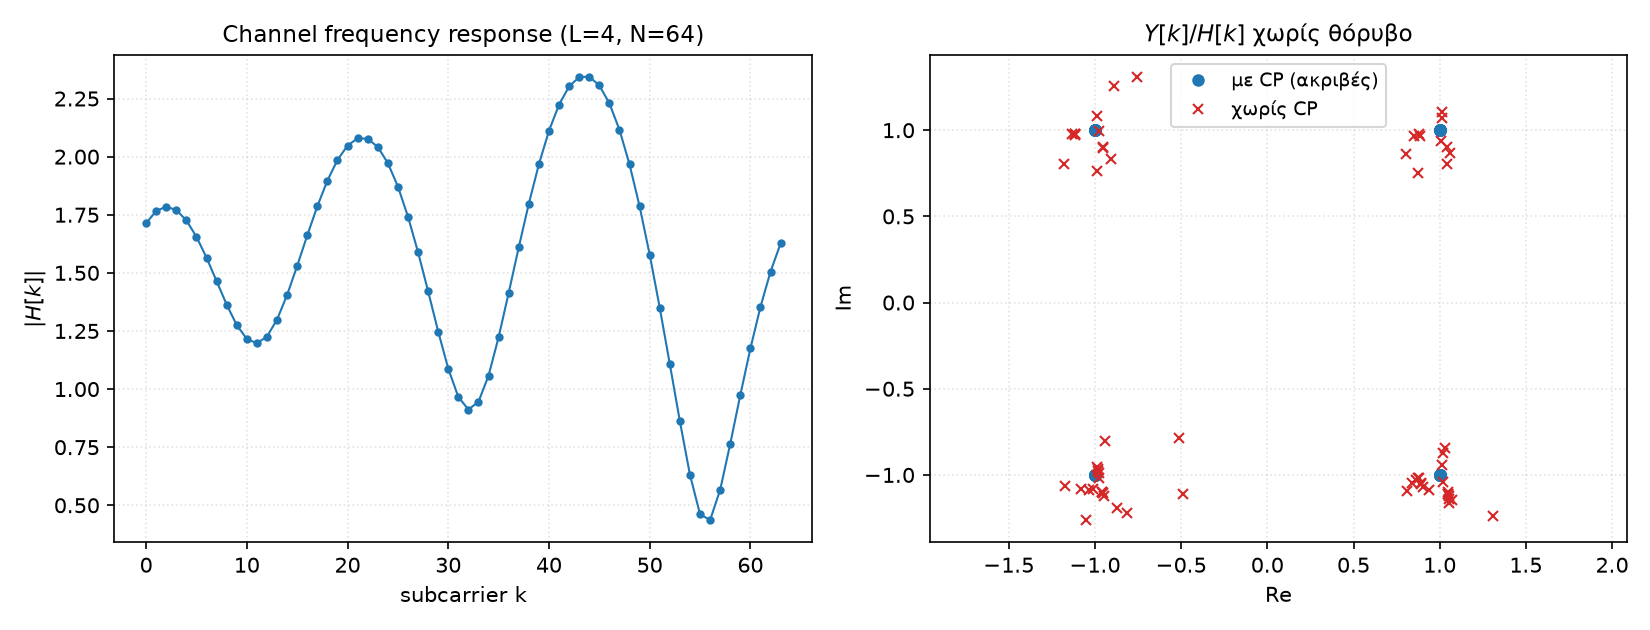
\includegraphics[width=0.92\textwidth]{B_flat_subchannels_N64.png}
  \caption{\en{Channel frequency response and the recovered constellation
  $\tilde y'_n/\tilde h_n$ in the noiseless case ($N_c=64$, $L=4$).}}
\end{figure}

Με \en{cyclic prefix} το σφάλμα είναι στο επίπεδο της ακρίβειας μηχανής ($\sim 10^{-15}$),
δηλαδή η εξ.~(4.14) ισχύει \emph{ακριβώς}. Το \en{frequency selective} κανάλι έχει πράγματι
μετατραπεί σε $N_c$ παράλληλα \en{flat} κανάλια, καθένα με έναν μιγαδικό συντελεστή
$\tilde h_n$ — αυτό ακριβώς απεικονίζει το Σχήμα~4.3 των σημειώσεων. Ισοδύναμα
$\tilde y'_n/\tilde h_n = \tilde d_n$ και ο αστερισμός ανακτάται τέλεια, όπως φαίνεται στο
δεξί υποσχήμα. Δεν απαιτείται δηλαδή \en{equalization}, παρά μόνο απόφαση σύμβολο προς
σύμβολο.

Χωρίς \en{cyclic prefix} το σφάλμα εκτοξεύεται στο $\sim 0.3$. Ο ρόλος του προθέματος είναι
ακριβώς να μετατρέψει τη \emph{γραμμική} συνέλιξη του καναλιού σε \emph{κυκλική} (εξ.~4.7),
ώστε ο \en{DFT} να τη διαγωνιοποιεί. Χωρίς αυτό εμφανίζεται \en{ISI} μεταξύ διαδοχικών
συμβόλων \en{OFDM} και απώλεια της ορθογωνιότητας των \en{subcarriers}. Το τίμημα είναι η
σχετική απώλεια $\frac{L-1}{N_c+L-1}$ σε χρόνο και ισχύ, που για $N_c=128$, $L=4$ είναι μόλις
$2.3\%$.

\subsection{Θόρυβος και θέσεις των σφαλμάτων ($\SNR = 15$~\dB{})}

\begin{zit}
Στην έξοδο του καναλιού, να προσθέσετε λευκό \en{Gaussian} θόρυβο ώστε να έχετε μέσο \SNR{}
(ενδεικτικά, $\SNR = 15$~\dB{}). Να συσχετίσετε τις θέσεις στις οποίες εμφανίζονται σφάλματα
απόφασης με αυτές στις οποίες το κανάλι έχει «μικρό» μέτρο απόκρισης συχνοτήτων. Τι
παρατηρείτε;
\end{zit}

Ο δέκτης εφαρμόζει \en{one-tap ZF} ανά \en{subcarrier},
$\hat{d}_n = \en{dec}\left(\tilde y'_n/\tilde h_n\right)$. Το πείραμα τρέχει για $N_c=128$,
$L=4$ και $4000$ πακέτα.

\begin{figure}[H]
  \centering
  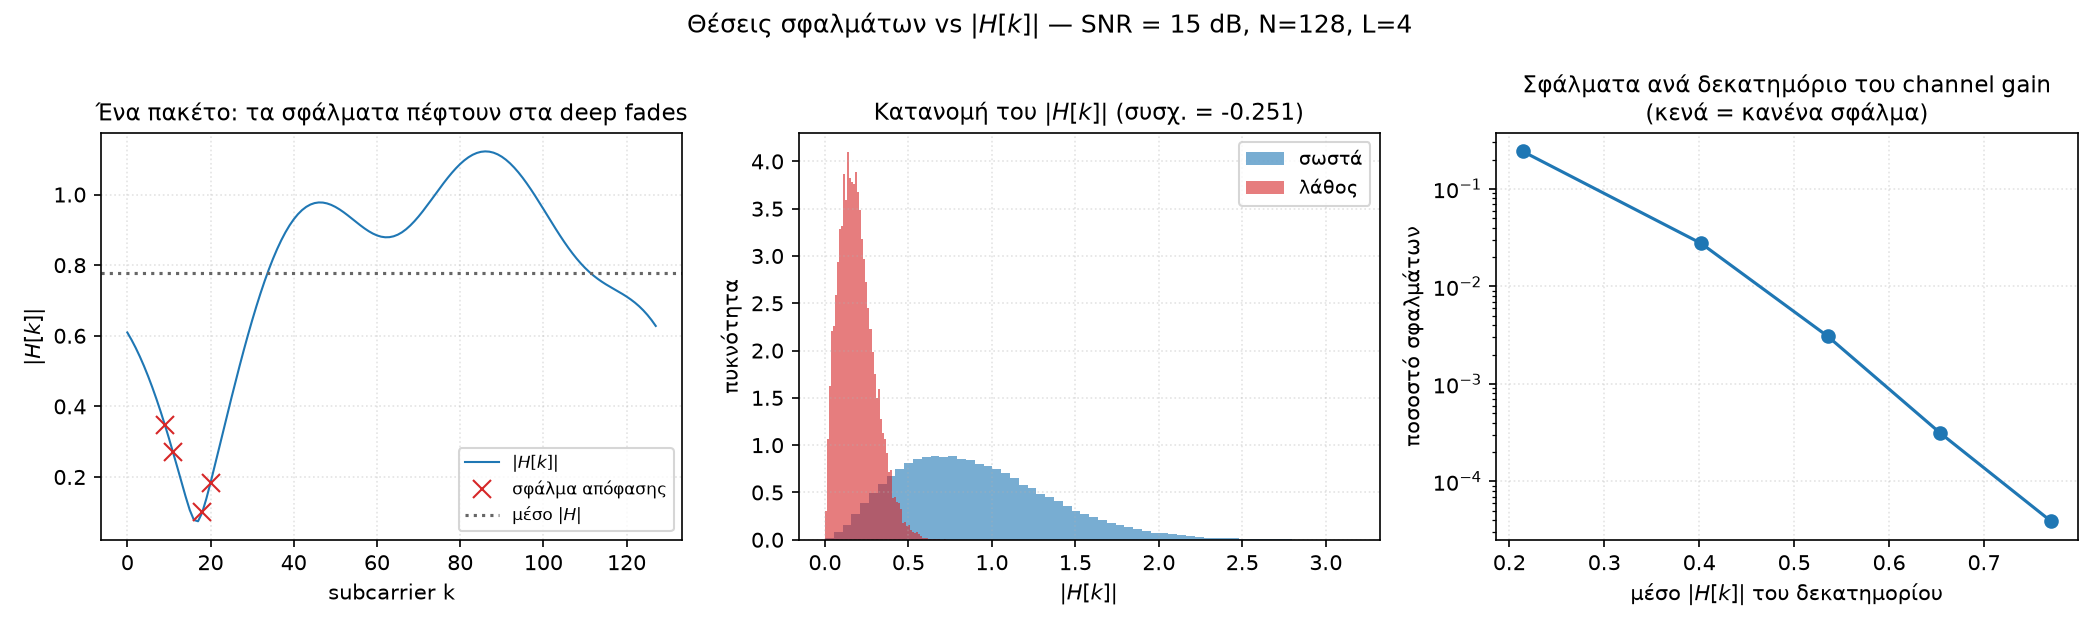
\includegraphics[width=\textwidth]{B_errors_vs_gain_SNR15.png}
  \caption{\en{Error positions versus $|\tilde h_n|$ at $\SNR = 15$~dB ($N_c=128$, $L=4$).}}
\end{figure}

\begin{table}[H]
  \centering\small
  \begin{tabular}{lc}
    \toprule
    Μέγεθος & Τιμή \\
    \midrule
    \en{Symbol error rate} ανά \en{subcarrier} & $0.0274$ \\
    Μέσο $|\tilde h_n|$ σε \textbf{σωστά} \en{subcarriers} & $0.903$ \\
    Μέσο $|\tilde h_n|$ σε \textbf{λανθασμένα} \en{subcarriers} & $0.192$ \\
    Συντελεστής συσχέτισης $|\tilde h_n| \leftrightarrow$ σφάλμα & $-0.251$ \\
    \bottomrule
  \end{tabular}
  \caption{\en{Correlation between decision errors and the channel gain.}}
\end{table}

\begin{table}[H]
  \centering\small
  \begin{tabular}{lccccc}
    \toprule
    δεκατημόριο του $|\tilde h_n|$ & $1$ο & $2$ο & $3$ο & $4$ο & $5$ο–$10$ο \\
    \midrule
    ποσοστό σφαλμάτων & $\mathbf{0.242}$ & $0.028$ & $0.003$ & $0.0004$ & $\approx 0$ \\
    \bottomrule
  \end{tabular}
  \caption{\en{Error rate per decile of $|\tilde h_n|$, from the weakest to the strongest.}}
\end{table}

Παρατηρούμε ότι τα σφάλματα δεν κατανέμονται ομοιόμορφα στα \en{subcarriers}:
συγκεντρώνονται σχεδόν αποκλειστικά εκεί όπου το κανάλι έχει \en{deep fade}. Το μέσο
$|\tilde h_n|$ στα λανθασμένα \en{subcarriers} είναι $4.7$ φορές μικρότερο από ό,τι στα
σωστά, ενώ το ασθενέστερο δεκατημόριο συγκεντρώνει ποσοστό σφαλμάτων $24.2\%$. Από το $4$ο
δεκατημόριο και πάνω πρακτικά δεν υπάρχουν σφάλματα, δηλαδή σχεδόν όλα τα σφάλματα
προέρχονται από το $\sim 20\%$ των \en{subcarriers} με το μικρότερο κέρδος.

Ο λόγος είναι ότι το στιγμιαίο \SNR{} του \en{subcarrier} $n$ είναι
$|\tilde h_n|^2 \cdot 2/\sigma_n^2$. Όπου το $|\tilde h_n|$ είναι μικρό, ο \en{one-tap ZF}
ενισχύει τον θόρυβο κατά $1/|\tilde h_n|$ και η απόφαση καταρρέει. Στο αριστερό υποσχήμα
φαίνεται καθαρά ένα μεμονωμένο πακέτο, όπου και τα τέσσερα σφάλματα πέφτουν μέσα στο
\en{fade} γύρω από το $n \approx 18$.

Το συμπέρασμα είναι ότι, χωρίς κωδικοποίηση ή \en{diversity}, το \BER{} ενός συστήματος
\en{OFDM} καθορίζεται από τα \emph{χειρότερα} \en{subcarriers} και όχι από το μέσο \SNR{}.
Αυτό ακριβώς κινητοποιεί το εδάφιο~4.2 των σημειώσεων και τα επόμενα ερωτήματα.

\subsection{Ανεξαρτησία φορέων (εδάφιο 4.2.1)}\label{sec:indep}

Πριν εφαρμόσουμε «επανάληψη στις συχνότητες» χρειάζεται να ξέρουμε \emph{ποιοι}
\en{subcarriers} φέρουν ανεξάρτητα κέρδη. Το εδάφιο~4.2.1 απαντά ακριβώς σε αυτό. Από την
εξ.~(4.20),
\[
  \mathbb{E}\!\left[\tilde h_i \tilde h_k^{*}\right]
  = \sigma_h^2 \sum_{l=0}^{L-1} e^{-j2\pi l (i-k)/N_c},
  \qquad \sigma_h^2 = \frac{1}{L},
\]
και, κατά την εξ.~(4.21), το άθροισμα μηδενίζεται όταν $i-k = c\,N_c/L$ με
$c = 1,\dots,L-1$. Επειδή τα $\tilde h_n$ είναι από κοινού κυκλικά \en{Gaussian},
ασυσχέτιστα σημαίνει και \emph{ανεξάρτητα}. Επαληθεύουμε την (4.20) αριθμητικά με
$2\cdot10^5$ υλοποιήσεις καναλιού για $N_c = 128$, $L = 4$ (άρα $N_c/L = 32$):

\begin{table}[H]
  \centering\small
  \begin{tabular}{cccc}
    \toprule
    $\Delta = i-k$ & θεωρία, εξ.~(4.20) & προσομοίωση & ασυσχέτιστοι; \\
    \midrule
    $1$  & $+0.9958-0.0735j$ & $+0.9965-0.0735j$ & όχι \\
    $2$  & $+0.9832-0.1458j$ & $+0.9839-0.1460j$ & όχι \\
    $16$ & $+0.2500-0.6036j$ & $+0.2500-0.6044j$ & όχι \\
    $32$ & $\phantom{+}0.0000+0.0000j$ & $-0.0002-0.0003j$ & \textbf{ναι} (εξ.~4.21) \\
    $64$ & $\phantom{+}0.0000+0.0000j$ & $-0.0001-0.0014j$ & \textbf{ναι} (εξ.~4.21) \\
    $96$ & $\phantom{+}0.0000+0.0000j$ & $-0.0016-0.0010j$ & \textbf{ναι} (εξ.~4.21) \\
    \bottomrule
  \end{tabular}
  \caption{\en{Sub-carrier correlation $\mathbb{E}[\tilde h_i \tilde h_k^{*}]$: theory
  (4.20) versus simulation ($N_c=128$, $L=4$).}}
\end{table}

Η συμφωνία θεωρίας και προσομοίωσης είναι πλήρης, και για $\Delta = 32, 64, 96$ η συσχέτιση
μηδενίζεται όπως προβλέπει η εξ.~(4.21). Γειτονικοί \en{subcarriers} ($\Delta = 1, 2$) είναι
αντίθετα σχεδόν τέλεια συσχετισμένοι — αυτή είναι η έννοια του \en{coherence bandwidth}
$W_c \approx W/L$ της εξ.~(4.17). Άρα η επανάληψη ενός συμβόλου σε $M \le L$
\en{subcarriers} με βήμα $N_c/M$ δίνει $M$ \emph{ανεξάρτητα} αντίγραφα.

\subsection{Διαφοροποίηση με «επανάληψη στις συχνότητες»}

\begin{zit}
Να χρησιμοποιήσετε επανάληψη στις συχνότητες για να εξάγετε \en{diversity} τάξης $1$, $2$ και
$4$. Να σχεδιάσετε το \BER{} για $\SNR_{\en{dB}} = [0:4:20]$. Να σχεδιάσετε την ποσότητα
$\log_{10}\SNR$ ως προς την ποσότητα $\log_{10}\BER$ και να προσπαθήσετε να επιβεβαιώσετε
ότι επιτυγχάνετε την επιδιωκόμενη τάξη \en{diversity} συγκρίνοντας γραφικά την κλίση του
γραφήματος με την κλίση κατάλληλα επιλεγμένων ευθειών γραμμών.
\end{zit}

Μεταδίδουμε το ίδιο σύμβολο \en{4-QAM} σε $M$ \en{subcarriers} με ανεξάρτητες υλοποιήσεις
καναλιού, $\tilde h_m \sim \mathcal{CN}(0,1)$, και τα συνδυάζουμε με \MRC{}:
\[
  r = \frac{h^{H} y}{\|h\|},
  \qquad
  y_m = \tilde h_m \tilde d + \tilde w_m,\ \ m=1,\dots,M .
\]

\begin{figure}[H]
  \centering
  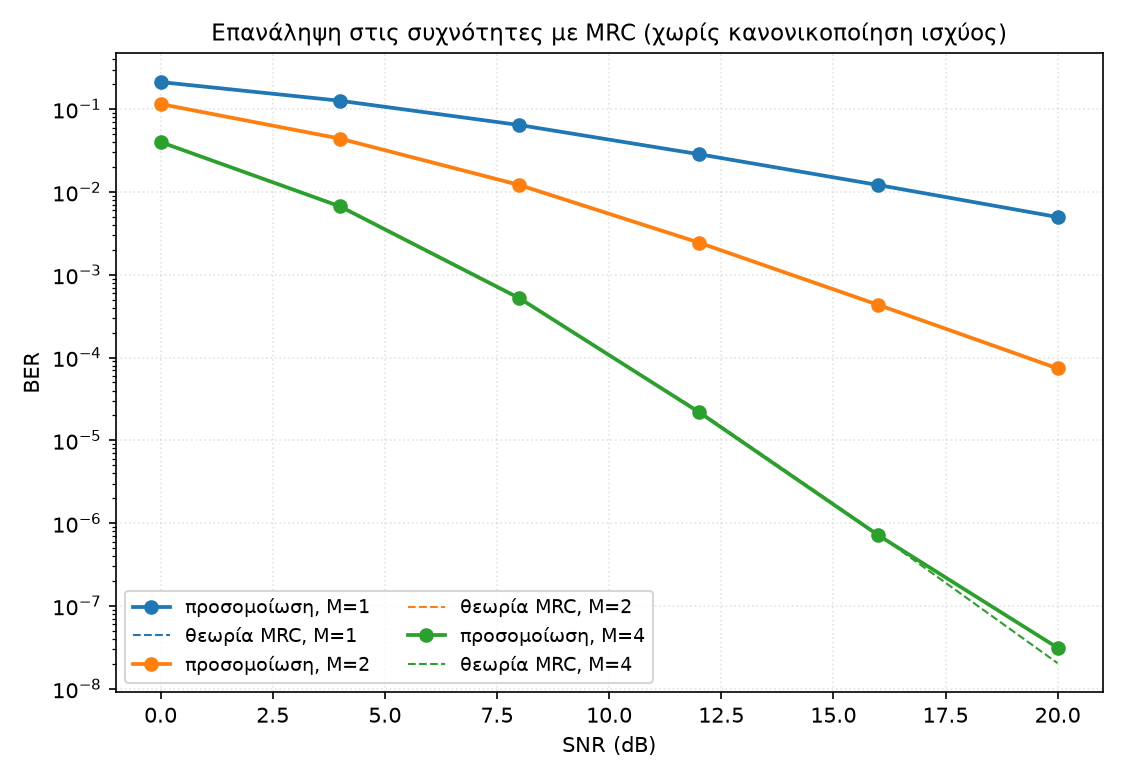
\includegraphics[width=0.49\textwidth]{B_repetition_ber_raw.png}%
  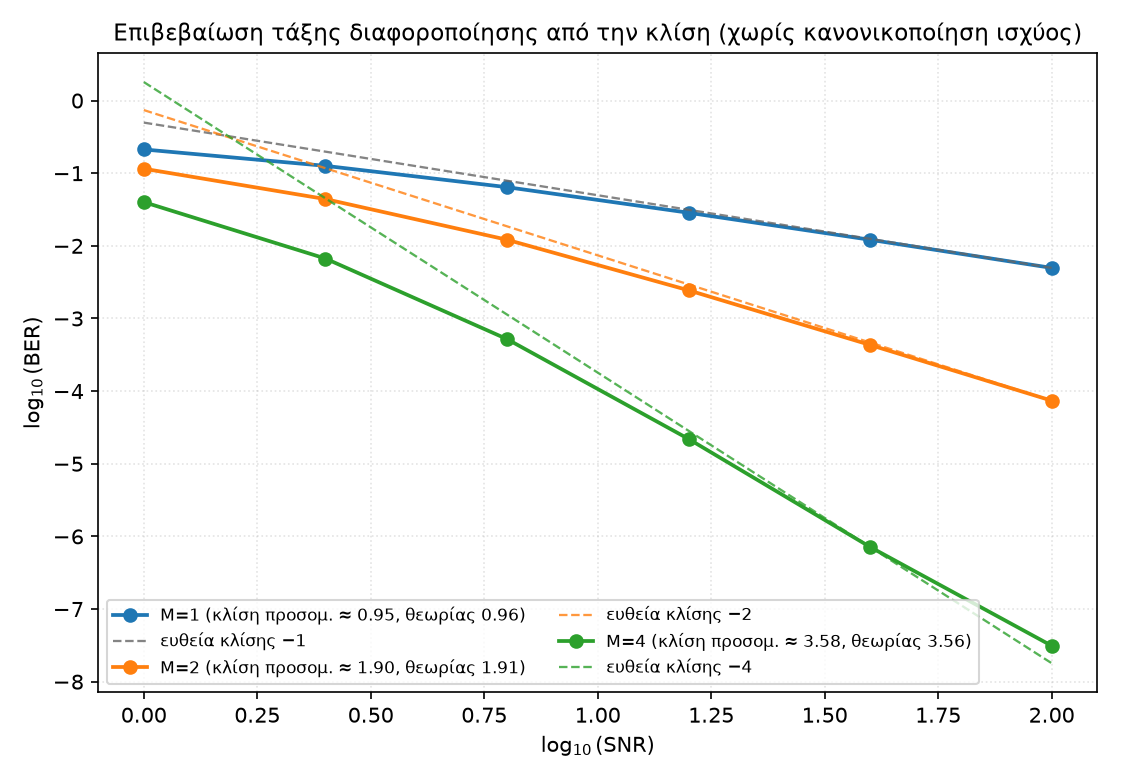
\includegraphics[width=0.49\textwidth]{B_repetition_loglog_raw.png}
  \caption{\en{Repetition in frequency with MRC. Left: BER versus SNR. Right:
  $\log_{10}\BER$ versus $\log_{10}\SNR$ together with reference lines of slope
  $-1$, $-2$, $-4$.}}
\end{figure}

\begin{table}[H]
  \centering\small
  \begin{tabular}{lcccccc}
    \toprule
    \SNR{} (\dB) & $0$ & $4$ & $8$ & $12$ & $16$ & $20$ \\
    \midrule
    $M=1$ & \texttt{2.12e-01} & \texttt{1.26e-01} & \texttt{6.43e-02} & \texttt{2.86e-02} & \texttt{1.21e-02} & \texttt{4.97e-03} \\
    $M=2$ & \texttt{1.15e-01} & \texttt{4.41e-02} & \texttt{1.21e-02} & \texttt{2.45e-03} & \texttt{4.32e-04} & \texttt{7.40e-05} \\
    $M=4$ & \texttt{4.00e-02} & \texttt{6.69e-03} & \texttt{5.21e-04} & \texttt{2.20e-05} & \texttt{7.16e-07} & \texttt{3.12e-08}$^{\dagger}$ \\
    \bottomrule
  \end{tabular}
  \caption{\en{BER for repetition of order $M = 1, 2, 4$.}}\label{tab:repideal}
\end{table}

\begin{table}[H]
  \centering\small
  \begin{tabular}{lccc}
    \toprule
    $M$ & κλίση προσομοίωσης & κλίση θεωρίας στο ίδιο παράθυρο & ασυμπτωτική τιμή \\
    \midrule
    $1$ & $0.95$ & $0.96$ & $1$ \\
    $2$ & $1.90$ & $1.91$ & $2$ \\
    $4$ & $3.58$ & $3.56$ & $4$ \\
    \bottomrule
  \end{tabular}
  \caption{\en{Measured slope of $\log_{10}\BER$ versus $\log_{10}\SNR$, compared with the
  theoretical MRC curve over the same SNR window.}}
\end{table}

Η επανάληψη σε $M$ \en{subcarriers} με ανεξάρτητα κέρδη δίνει τάξη \en{diversity} $M$, όπως
ακριβώς προβλέπει το εδάφιο~4.2: το σύμβολο χάνεται μόνο αν \emph{όλα} τα $M$ αντίγραφα
βρεθούν ταυτόχρονα σε \en{fade}. Το κέρδος είναι τεράστιο στα υψηλά \SNR{}: στα $20$~\dB{}
το \BER{} πέφτει από $4.97\cdot10^{-3}$ ($M=1$) σε $3.12\cdot10^{-8}$ ($M=4$), δηλαδή πέντε
τάξεις μεγέθους. Στο γράφημα $\log_{10}\BER$ ως προς $\log_{10}\SNR$ οι καμπύλες γίνονται
ευθείες με κλίσεις που πλησιάζουν τις ευθείες αναφοράς $-1$, $-2$ και $-4$. Το τίμημα, όπως
σημειώνουν και οι σημειώσεις, είναι ότι ο ρυθμός μετάδοσης μειώνεται $M$ φορές.

Αξίζει να σχολιάσουμε γιατί η κλίση για $M=4$ είναι $3.58$ και όχι $4$. Όπως και στο πρώτο
μέρος, η τάξη \en{diversity} είναι ασυμπτωτική έννοια: η \emph{ίδια η θεωρητική} καμπύλη
\MRC{} έχει κλίση $3.56$ στο ίδιο παράθυρο \SNR{} και φτάνει το $4.00$ μόνο πέρα από τα
$\sim 35$~\dB{}. Η συμφωνία προσομοίωσης και θεωρίας σε δύο δεκαδικά ψηφία είναι η ουσιαστική
επαλήθευση, και όχι η απόσταση από τον ακέραιο $M$. Στο εύρος $0{:}4{:}20$~\dB{} της
εκφώνησης η ασυμπτωτική περιοχή απλώς δεν έχει ακόμη κατακτηθεί για $M=4$.

\subsection{Επανάληψη μέσα σε πραγματικό σύμβολο \en{OFDM} με βήμα $N_c/M$}

Το παραπάνω πείραμα υποθέτει \emph{εξ ορισμού} ανεξάρτητα αντίγραφα. Η θεωρία του εδαφίου
4.2 όμως λέει κάτι ισχυρότερο: ότι τα ανεξάρτητα αντίγραφα προκύπτουν \emph{από το ίδιο το
κανάλι}, αρκεί να τοποθετηθούν σε \en{subcarriers} με απόσταση $N_c/M$
(εδάφιο~\ref{sec:indep}). Το επαληθεύουμε στήνοντας ολόκληρη την αλυσίδα \en{OFDM} —
$\en{IDFT} \to \CP{} \to$ γραμμική συνέλιξη με το κανάλι $\to$ θόρυβος $\to$ αφαίρεση
\CP{} $\to \en{DFT}$ — και φορτώνοντας κάθε σύμβολο σε $M$ \en{subcarriers} με βήμα $N_c/M$,
τα οποία συνδυάζουμε με \MRC{} πάνω στα $\tilde y'_n$ της εξ.~(4.14). Εδώ, για $N_c=128$ και
$L=4$, το βήμα είναι $128$, $64$ και $32$ φορείς για $M = 1, 2, 4$ αντίστοιχα.

\begin{figure}[H]
  \centering
  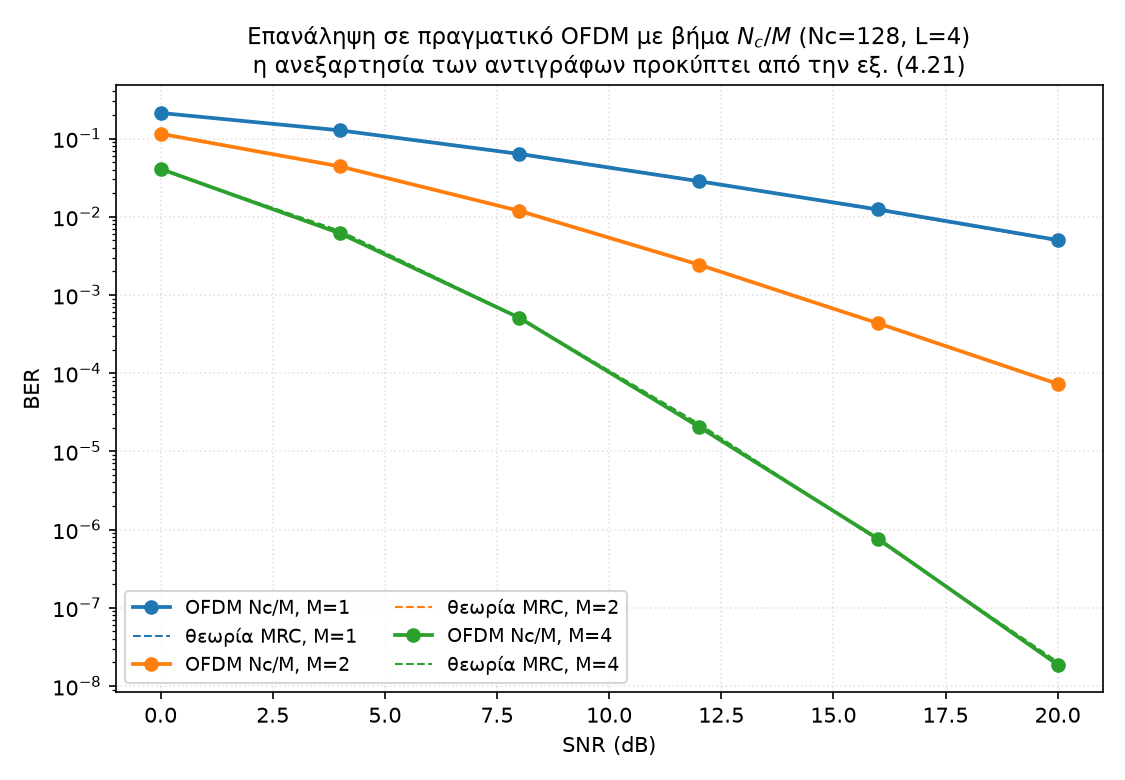
\includegraphics[width=0.78\textwidth]{B_ofdm_repetition_Nc128.png}
  \caption{\en{Repetition inside a real OFDM symbol, copies spaced $N_c/M$ sub-carriers
  apart ($N_c=128$, $L=4$).}}
\end{figure}

\begin{table}[H]
  \centering\small
  \begin{tabular}{lcccccc c}
    \toprule
    \SNR{} (\dB) & $0$ & $4$ & $8$ & $12$ & $16$ & $20$ & κλίση \\
    \midrule
    $M=1$ & \texttt{2.12e-01} & \texttt{1.27e-01} & \texttt{6.35e-02} & \texttt{2.85e-02} & \texttt{1.24e-02} & \texttt{5.04e-03} & $0.94$ \\
    $M=2$ & \texttt{1.15e-01} & \texttt{4.40e-02} & \texttt{1.19e-02} & \texttt{2.44e-03} & \texttt{4.34e-04} & \texttt{7.29e-05} & $1.91$ \\
    $M=4$ & \texttt{4.09e-02} & \texttt{6.13e-03} & \texttt{5.10e-04} & \texttt{2.07e-05} & \texttt{7.59e-07} & \texttt{1.88e-08}$^{\dagger}$ & $3.53$ \\
    \bottomrule
  \end{tabular}
  \caption{\en{BER of repetition inside a real OFDM symbol with spacing $N_c/M$.}}
\end{table}

Η σύμπτωση με τον Πίνακα~\ref{tab:repideal} είναι αξιοσημείωτη: σε κάθε \SNR{} και για κάθε $M$ τα δύο
πειράματα συμφωνούν στο δεύτερο σημαντικό ψηφίο (π.χ. στα $20$~\dB{} για $M=2$,
$7.29\cdot10^{-5}$ έναντι $7.40\cdot10^{-5}$), και οι κλίσεις είναι $0.94$, $1.91$, $3.53$
έναντι $0.95$, $1.90$, $3.58$. Δηλαδή δεν χρειάστηκε να \emph{υποθέσουμε} ανεξάρτητα
αντίγραφα: η ανεξαρτησία προέκυψε από το ίδιο το κανάλι, ακριβώς όπως προβλέπει η εξ.~(4.21).
Αυτή είναι και η ουσιαστικότερη επαλήθευση του εδαφίου~4.2 των σημειώσεων.

Σημειώνουμε ότι η επιλογή $M \le L$ δεν είναι τυχαία: το κανάλι έχει μόνο $L$ ανεξάρτητους
βαθμούς ελευθερίας στη συχνότητα, οπότε $M = L = 4$ είναι η μέγιστη τάξη \en{diversity} που
μπορεί να εξαχθεί με επανάληψη μέσα σε ένα σύμβολο \en{OFDM}.

\subsubsection*{\en{Diversity gain} έναντι \en{array gain}}

Στα παραπάνω κάθε αντίγραφο εκπέμπεται με πλήρη ισχύ, οπότε το $M=4$ απολαμβάνει ταυτόχρονα
\en{diversity gain} (κλίση) και \en{array gain} (οριζόντια μετατόπιση κατά
$10\log_{10}M$~\dB{}). Για πληρότητα τρέξαμε και τη «δίκαιη» εκδοχή, όπου η συνολική ισχύς
μοιράζεται στα $M$ αντίγραφα.

\begin{figure}[H]
  \centering
  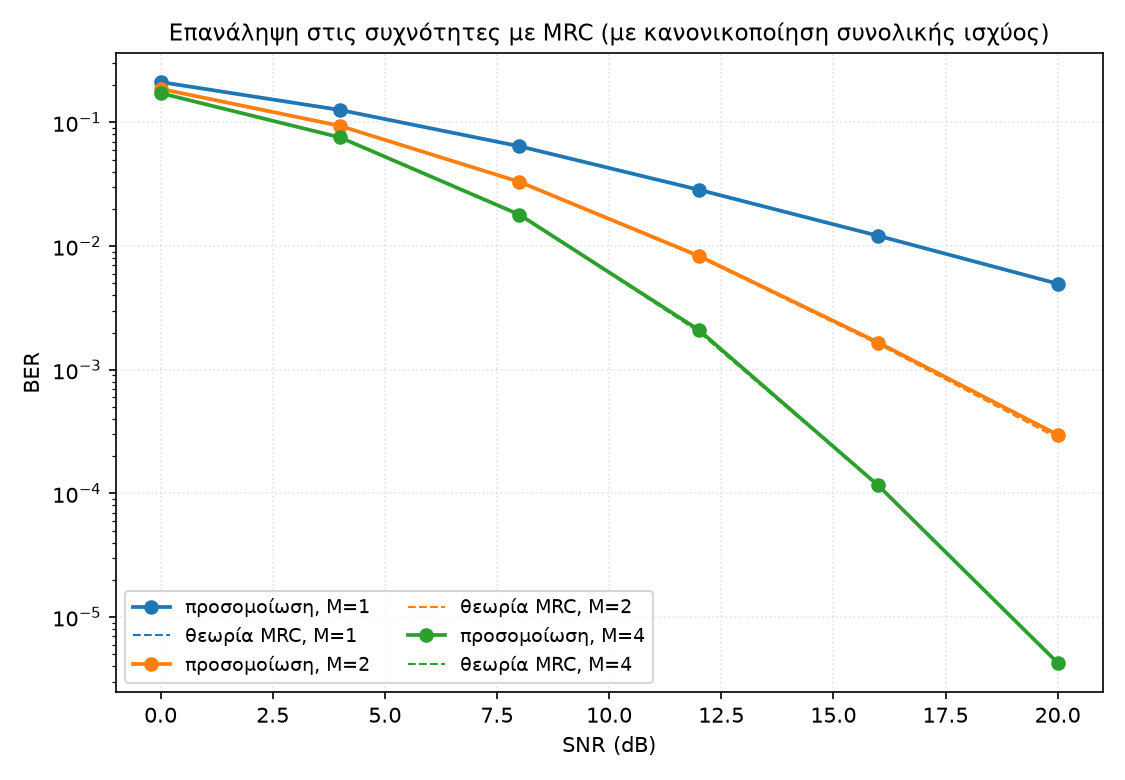
\includegraphics[width=0.49\textwidth]{B_repetition_ber_norm.png}%
  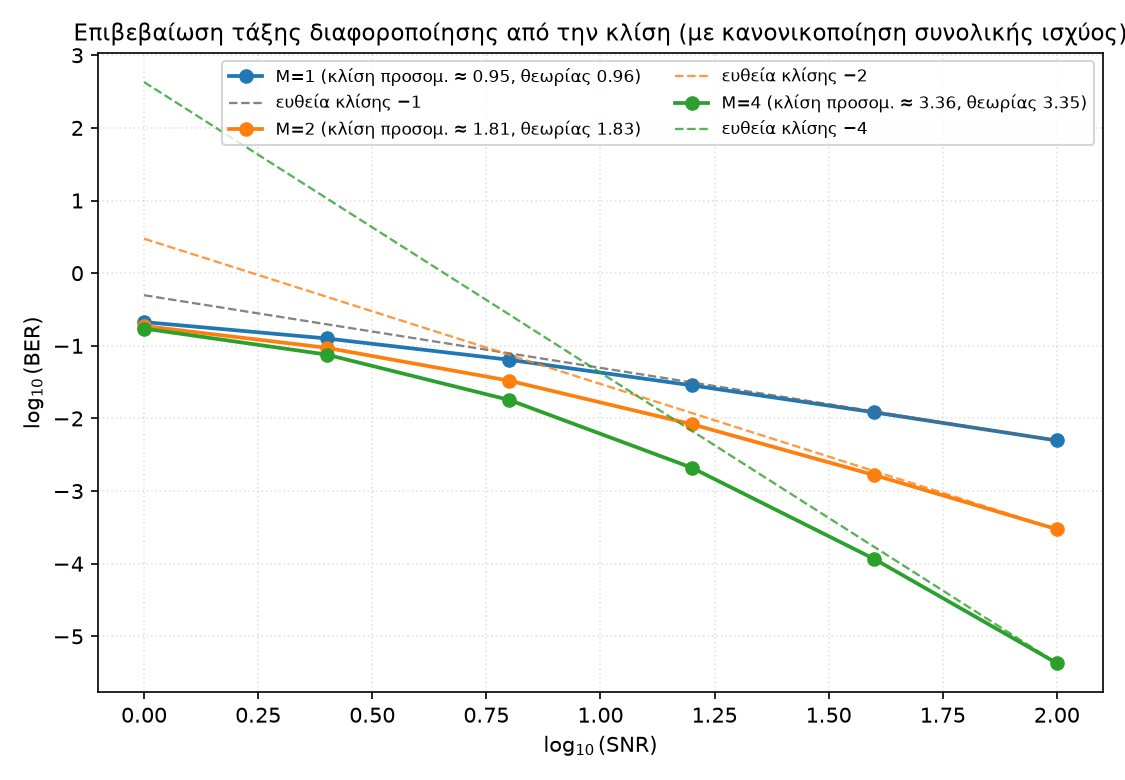
\includegraphics[width=0.49\textwidth]{B_repetition_loglog_norm.png}
  \caption{\en{Same experiment with the total transmit power shared among the $M$ copies.}}
\end{figure}

\begin{table}[H]
  \centering\small
  \begin{tabular}{lccc}
    \toprule
    $M$ & \BER{} στα $20$~\dB{} (πλήρης ισχύς) & \BER{} στα $20$~\dB{} (μοιρασμένη ισχύς)
        & κλίση (μοιρ.) / θεωρία \\
    \midrule
    $1$ & \texttt{4.97e-03} & \texttt{4.97e-03} & $0.95$ / $0.96$ \\
    $2$ & \texttt{7.40e-05} & \texttt{2.98e-04} & $1.81$ / $1.83$ \\
    $4$ & \texttt{3.12e-08} & \texttt{4.27e-06} & $3.36$ / $3.35$ \\
    \bottomrule
  \end{tabular}
  \caption{\en{Full transmit power per copy versus shared total power.}}
\end{table}

Ακόμη και με σταθερή συνολική ισχύ το κέρδος παραμένει τεράστιο ($4.97\cdot10^{-3}$ σε
$4.27\cdot10^{-6}$ στα $20$~\dB{}), γεγονός που δείχνει ότι η βελτίωση οφείλεται πράγματι στο
\en{diversity} και όχι απλώς σε περισσότερη εκπεμπόμενη ενέργεια.

% =====================================================================
\section{Συμπεράσματα}

\begin{enumerate}[leftmargin=2em]
  \item Ο δέκτης \Rake{} εξάγει το \en{frequency diversity} του καναλιού. Με $L$
        \en{fingers} πετυχαίνει τάξη \en{diversity} $L$, ταυτιζόμενος με την εξ.~(4.16) των
        σημειώσεων και με τη θεωρία \MRC{}.
  \item Οι προσεγγίσεις (4.11) και (4.14) του κεφαλαίου είναι θεμιτές για $L \ll N$: η
        υπολειπόμενη συσχέτιση των ολισθημένων \en{codes} κλιμακώνεται ως $1/\sqrt{N}$ και η
        προσομοίωση με πλήρη γραμμική συνέλιξη πέφτει πάνω στη θεωρητική καμπύλη.
  \item Το \en{selection combining} κρατά την τάξη \en{diversity} αλλά χάνει \en{array gain}
        (περίπου $3$~\dB{} για $L=3$): σημαντικά απλούστερος δέκτης με μετρήσιμο τίμημα.
  \item Το \en{DS-CDMA} είναι \en{interference-limited} και όχι \en{noise-limited}. Τα τυχαία
        \en{codes} δεν είναι ορθογώνια, οπότε δεν ισχύει η ιδανική εξ.~(4.9), εμφανίζεται
        \en{error floor} και το \en{diversity} εξαφανίζεται. Το φάρμακο είναι μεγαλύτερο
        \en{processing gain} $N$ ή \en{multi-user detection}.
  \item Το \en{cyclic prefix} είναι αυτό που κάνει το \en{OFDM} να δουλεύει: μετατρέπει τη
        γραμμική συνέλιξη σε κυκλική (εξ.~4.7) και το \en{frequency selective} κανάλι σε
        $N_c$ \en{flat} κανάλια με ακρίβεια μηχανής, με τίμημα μόλις
        $\frac{L-1}{N_c+L-1} = 2.3\%$.
  \item Το \en{OFDM} από μόνο του δεν δίνει \en{diversity}. Τα σφάλματα συγκεντρώνονται στα
        \en{subcarriers} με \en{deep fade} και χρειάζεται επανάληψη (ή κωδικοποίηση) στις
        συχνότητες. Η εξ.~(4.21) μάς λέει ακριβώς πού να τοποθετήσουμε τα αντίγραφα: σε
        απόσταση $N_c/L$ — και η προσομοίωση σε πραγματικό \en{OFDM} το επιβεβαιώνει.
  \item Η τάξη \en{diversity} είναι ασυμπτωτική έννοια. Οι μετρούμενες κλίσεις σε πεπερασμένο
        \SNR{} είναι συστηματικά μικρότερες από τον ακέραιο στόχο — το ίδιο ισχύει και για
        τις θεωρητικές καμπύλες, με τις οποίες συμφωνούν σε δύο δεκαδικά ψηφία.
\end{enumerate}

\end{document}
